\section{Structure Prediction by Sequence Homology. Searching for Homologues}
\label{sec:structurePrediction}
As we have mentioned above, in this tutorial we are going to use tools that allow to predict the atomic structure from sequence homology. 

Structure prediction by sequence homology only requires the sequence itself of the specimen that we would like to model, from now ahead the \iii{target sequence}, and the access to databases to seek structures or \iii{templates} of homologous molecules. The sequences of homologous molecules show statistically significant similarity because they share common ancestry. Since the sequence encodes the structural information, from high similar sequences necessarily follows high similar structures. Structures from the nearest homologous molecules will thus be preferred over remote relative ones. Remark that molecules containing several domains usually require independent searching for homologous templates of each domain. A small review about sequence similarity searching can be found in \citep{pearson2013}, and in \citep{kryshtafovych2018} the assessment of current \iii{template}-based modeling methods, many of them implemented as fully automated servers. Modeling tools appropriate to search for remote homologous \iii{templates}, folding recognition and \iii{template}-free methods (\iii{ab initio}), as well as $de\ novo$ modeling tools, which besides sequences use the volume itself, have still to be included in \scipion framework. 


\subsubsection*{How to identify \iii{templates} of the \iii{target sequence}}
 Similarity searching programs like \ttt{BLAST} (\ffigure{fig:blastp}) \citep{altschul1997}, available in \url{https://blast.ncbi.nlm.nih.gov/Blast.cgi}, use the \iii{target sequence} (1) to screen the structure-containing database \ttt{PDB} (2). Selecting or excluding a particular organism is an option (3). We usually start our searching selecting the organism in which we are interested or the closest evolutionarily related ones. If no similar sequences are found in these organisms, unrelated organisms may be selected or no one at all. Different searching algorithms are available (4) and one of them has to be selected. After executing \ttt{BLAST} (5) a list of score-ordered \iii{templates} is retrieved. 
 
  \begin{figure}[H]
  \centering 
  \captionsetup{width=.7\linewidth} 
  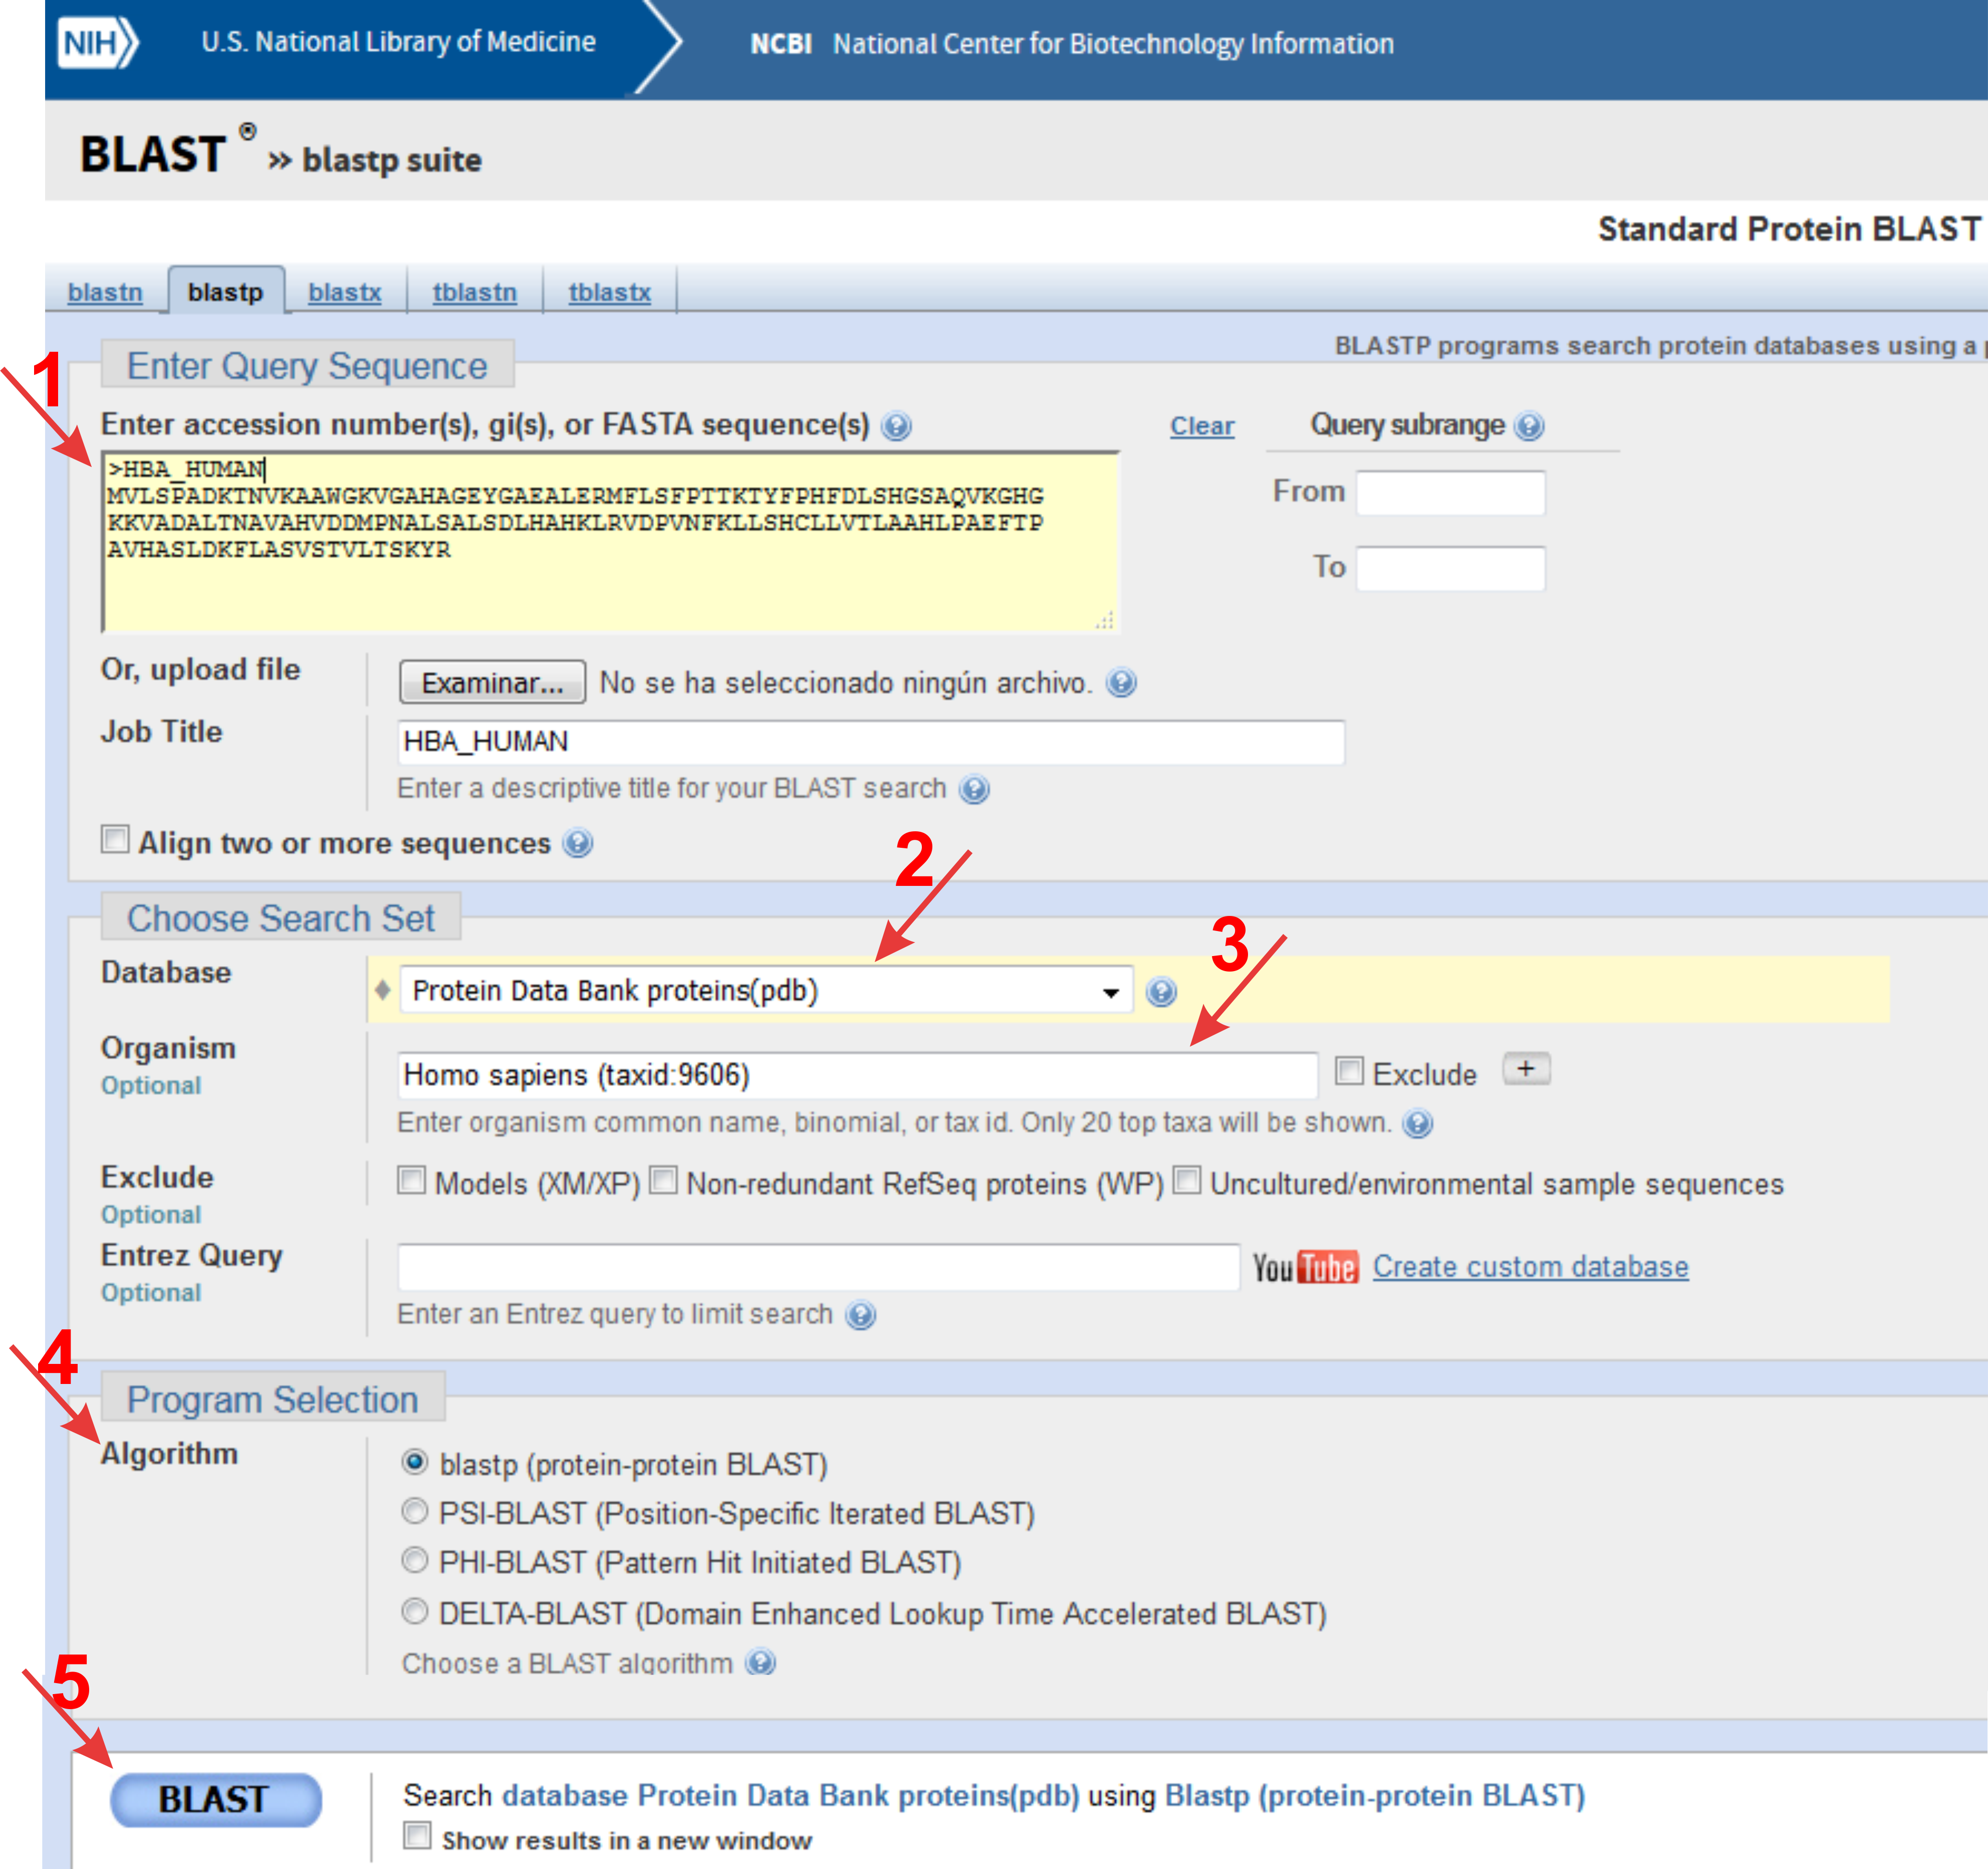
\includegraphics[width=0.80\textwidth]{Images/Fig9}
  \caption{Form of the similarity searching program \ttt{BLAST}.}
  \label{fig:blastp}
  \end{figure}
  
  Of course, the closest relatives to human \ttt{Hgb} subunits, structurally characterized, will be their own structures contained in \ttt{PDB-5NI1}. However, in this tutorial we are going to assume that in our example the closest relatives to the human \ttt{Hgb} $\alpha$ and $\beta$ subunits are the respective \ttt{Hgb} subunits (identity 49.3\% and 45.21\%) of the antarctic fish \iii{Pagothenia bernacchii} \citep{camardella1992}. The atomic structure associated to this \iii{template} has \ttt{PDB} accession code \ttt{1PBX}. Information about the structure can be checked in \url{https://www.rcsb.org/structure/1PBX}. In general, it is a good idea to read the information related with the \iii{template}, do it so and answer the following questions: (Answers in appendix \ref{app:solutions}; \textbf{Question \ref{sec:structurePrediction}\_1})
  
  \begin{minipage}{\linewidth}
    \begin{framed}
      \begin{itemize}
        \item How has this structure been obtained (X-ray diffraction, EM, NMR)?
        \item What resolution does it have?
        \item How many chains does it include?
      \end{itemize}
    \end{framed}
  \end{minipage}
\\
\\
  
  \ttt{NOTE}: \chimera also incorporates the possibility of run the \ttt{BLAST} algoritnm, although with lower number of options than those shown in \ffigure{fig:blastp}. Nevertheless, if you know that there are high similar homologous sequences with associated structure, you can skip this searching step ``outside'' \scipion and go to the next step to get directly your  \iii{template} and your \iii{target model}.  
